\documentclass[12pt, oneside]{article}
\usepackage[letterpaper, margin=1.2in, headsep=0.7in]{geometry}
\usepackage[english]{babel}
\usepackage[utf8]{inputenc}
\usepackage{amsmath}
\usepackage{amsfonts}
\usepackage{amssymb}
\usepackage{tikz}
\usepackage{venndiagram}

\usepackage{fancyhdr}
\pagestyle{fancy}
\fancyhf{}
\rhead{Name: \hspace{.75in} }
\lhead{BECA / Dr. Huson / Geometry \\* 19 November 2018 \\* Homework: Algebra \& graphing review}

\renewcommand{\headrulewidth}{0pt}

\title{Worksheet and test template}
\author{Chris Huson}
\date{February 2018}

\begin{document}

Simplify by collecting like terms.

\begin{enumerate}


\item $2x^2+13x -12 -2x^2-3x+5$\\*[40pt]
\item $3(a^2-2a +7) -2(a^2-3a-10)$\\*[60pt]
\item $(a +7)(3a-1)$\\*[50pt]


Solve for the value of $x$.
\item   $-9= \frac{3}{4}x$\\*[60pt]
\item   $\frac{2}{3}(3x-6)=-2x$\\*[60pt]


What is the slope and $y$-intercept of each equation?
\item   $y=-3.4x-1.8$\\*[20pt]
\item   $5x+2y=8$

\newpage
Use pencil for graphs. Label each function with its name or equation.
\item Given the function $f(x)=\frac{2}{5}x-5$.
\begin{enumerate}
    \item Draw the function $f(x)$ on the graph below.
    \item Mark and label the point $P (3, 2)$ on the graph.
    \item A second line, $g(x)$, is perpendicular to $f(x)$ and passes through point $P$. Plot $g(x)$ on the graph.
    \item Challenge: what is the exact value of the $y$-intercept of $g(x)$?\\*[10pt]
\end{enumerate}

\begin{figure}[!ht]
    \centering
    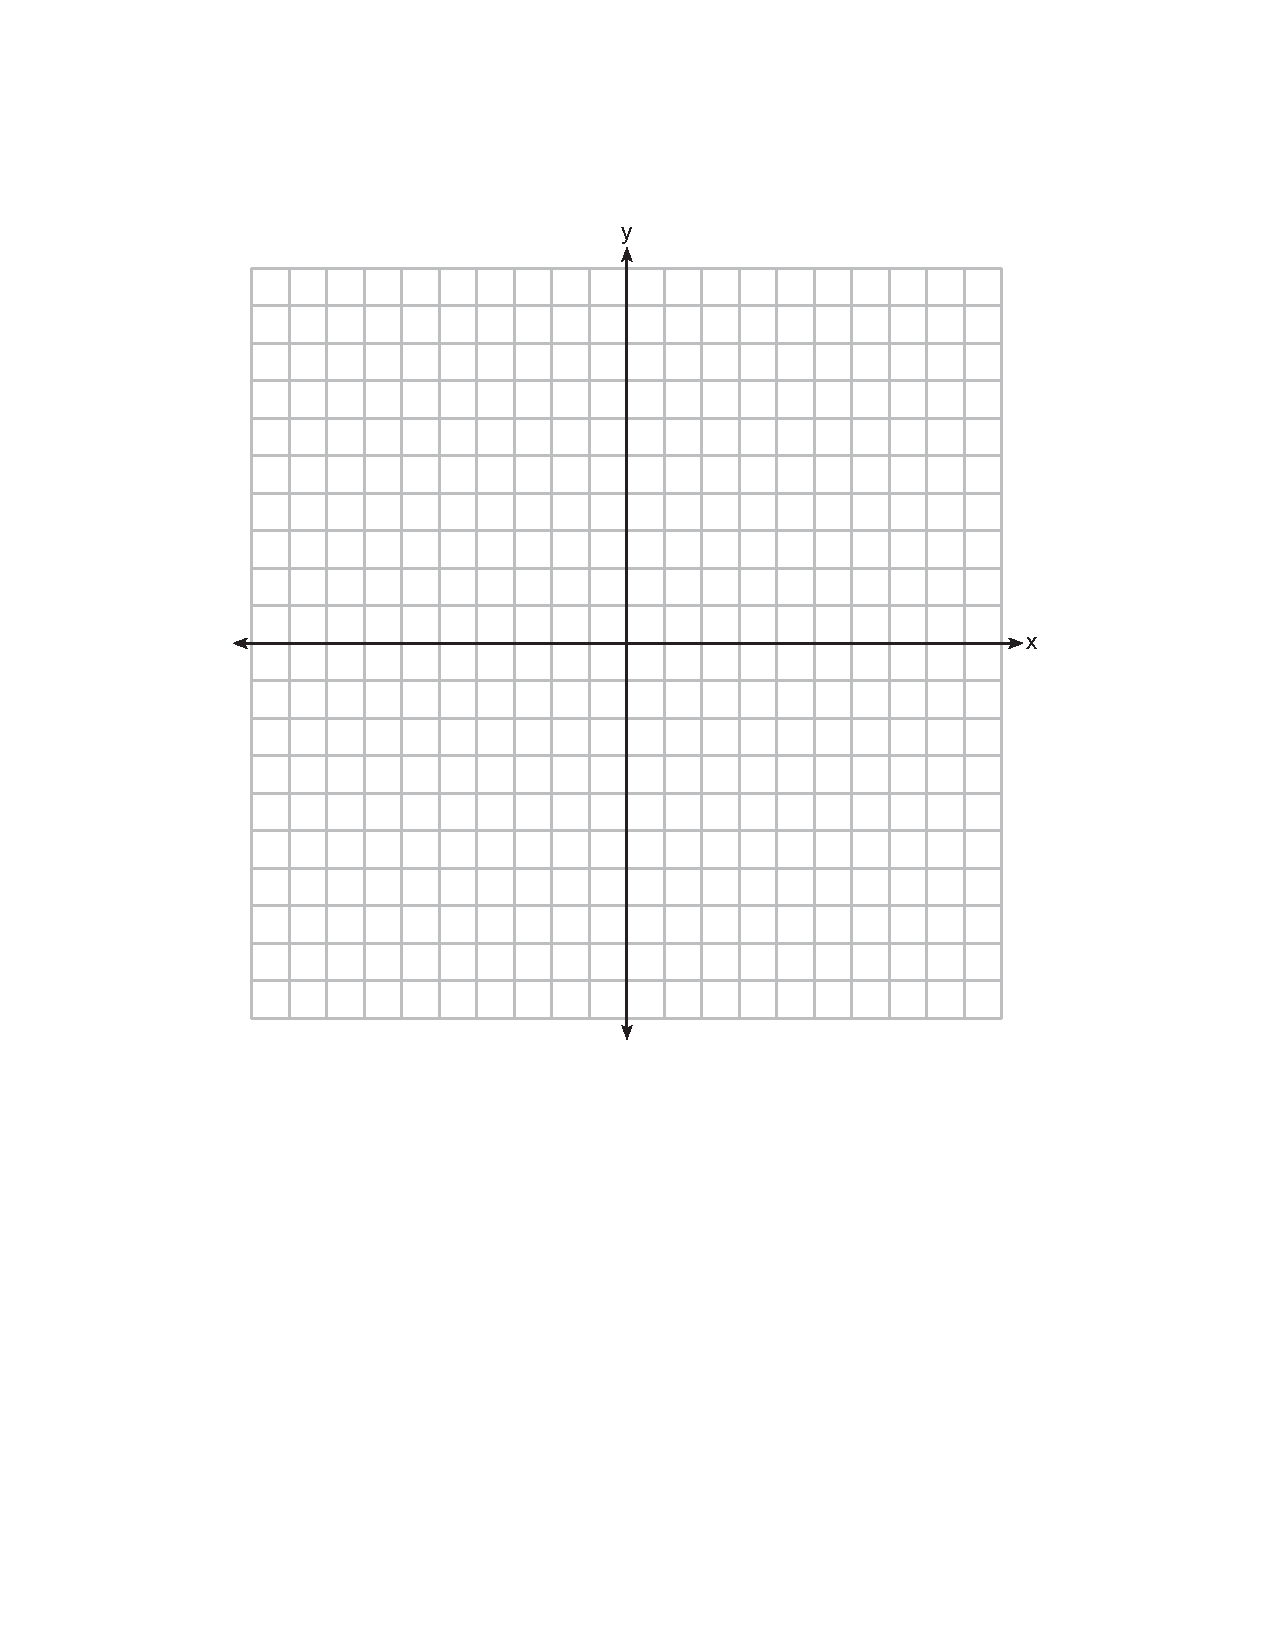
\includegraphics[width=0.75\textwidth]{regents-grid.pdf}
\end{figure}

\newpage

\item Explain why the radical $\sqrt[3]{5^2}$ is equivalent to $25^{\frac{1}{3}}$, an expression with a rational exponent.\\*[60pt]

\item Solve the system of equations by graphing. Select a point in the solution set and label it on the graph as ordered pair.
\[x+4y \geq -8\]
\[y < \frac{1}{2}x-4\]

\begin{figure}[!ht]
    \centering
    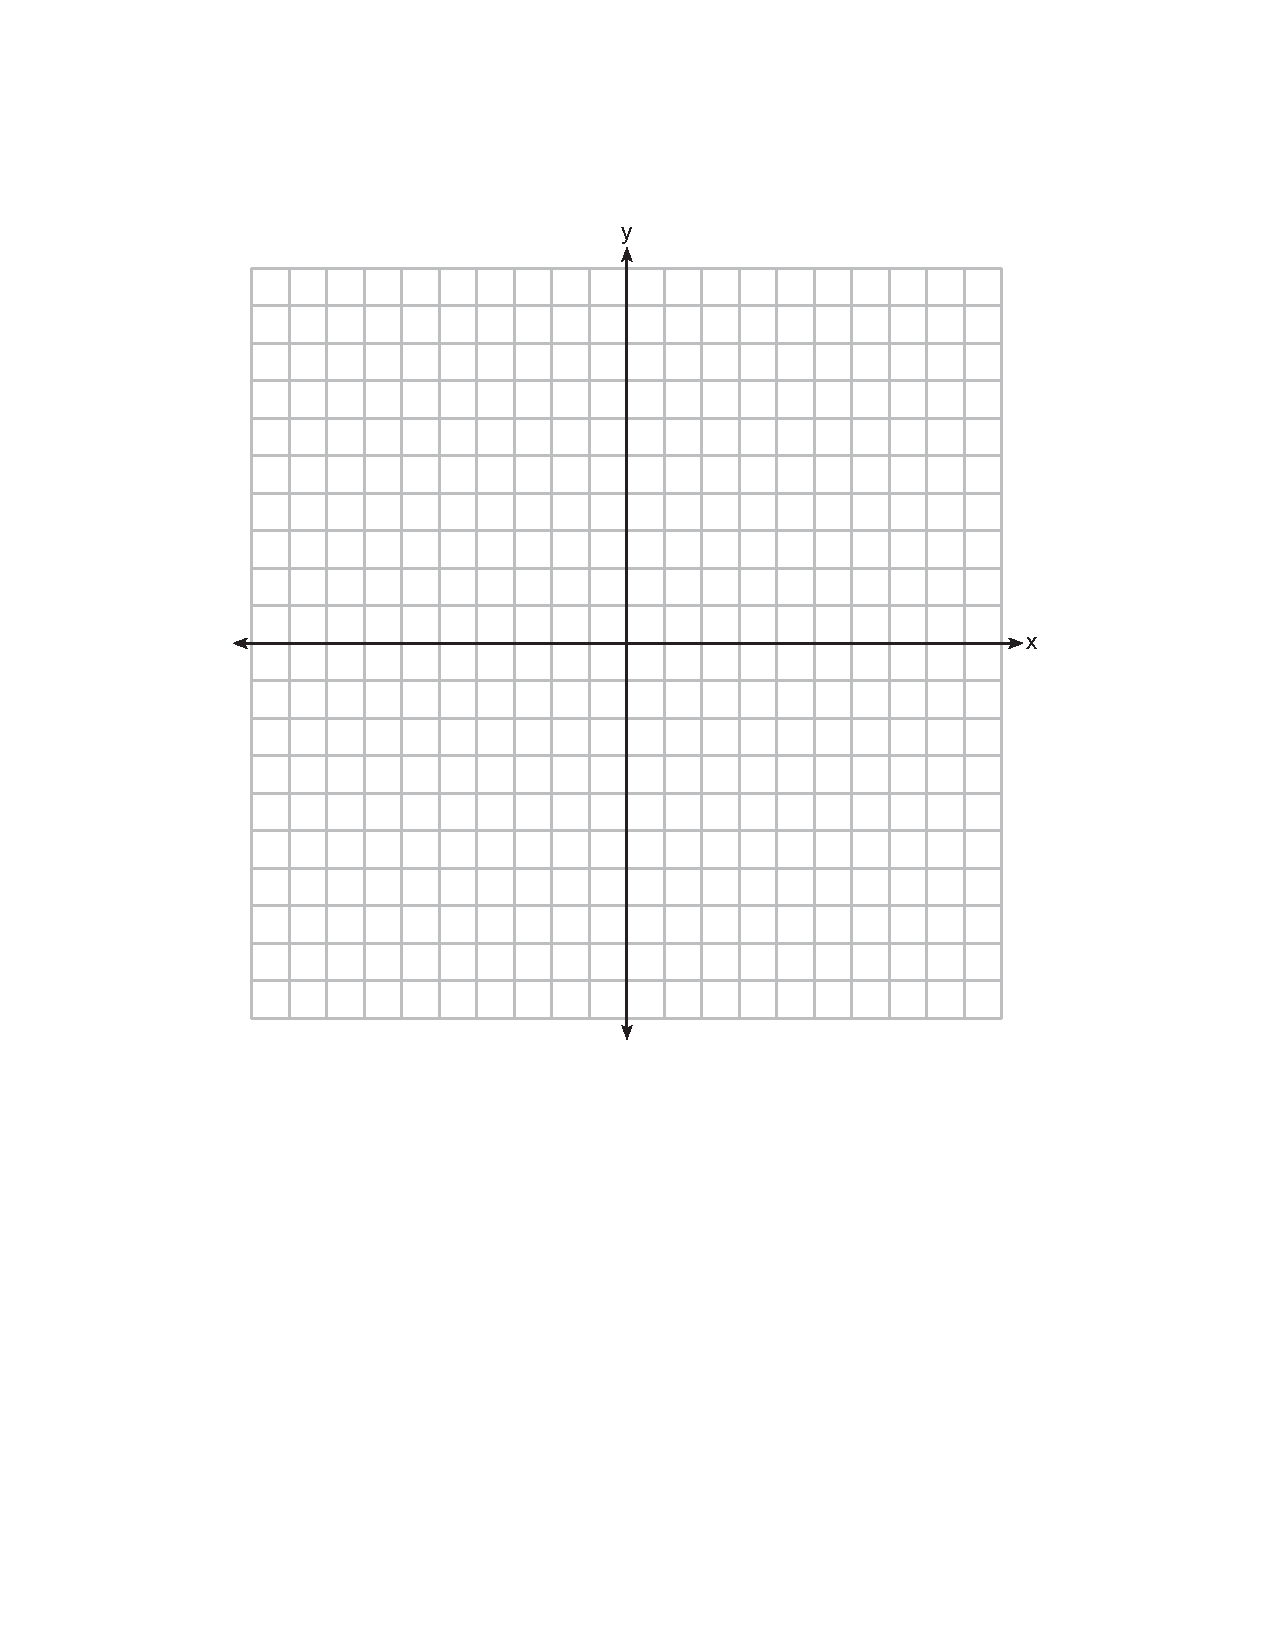
\includegraphics[width=0.65\textwidth]{regents-grid.pdf}
\end{figure}

Solve the system algebraically.
\item
$3x+4y=15$\\*
$3x+y=3$

\newpage
\item Given the function $f(x)=x^2-x-12$.
\begin{enumerate}
    \item Make a table of $x$ values from -5 to +5 versus $f(x)$
    \item Draw the function $f(x)$ on the graph below.
    \item Challenge: what is the exact value of the $y$-intercept of $g(x)$?\\*[10pt]
\end{enumerate}

\begin{figure}[!ht]
    \centering
    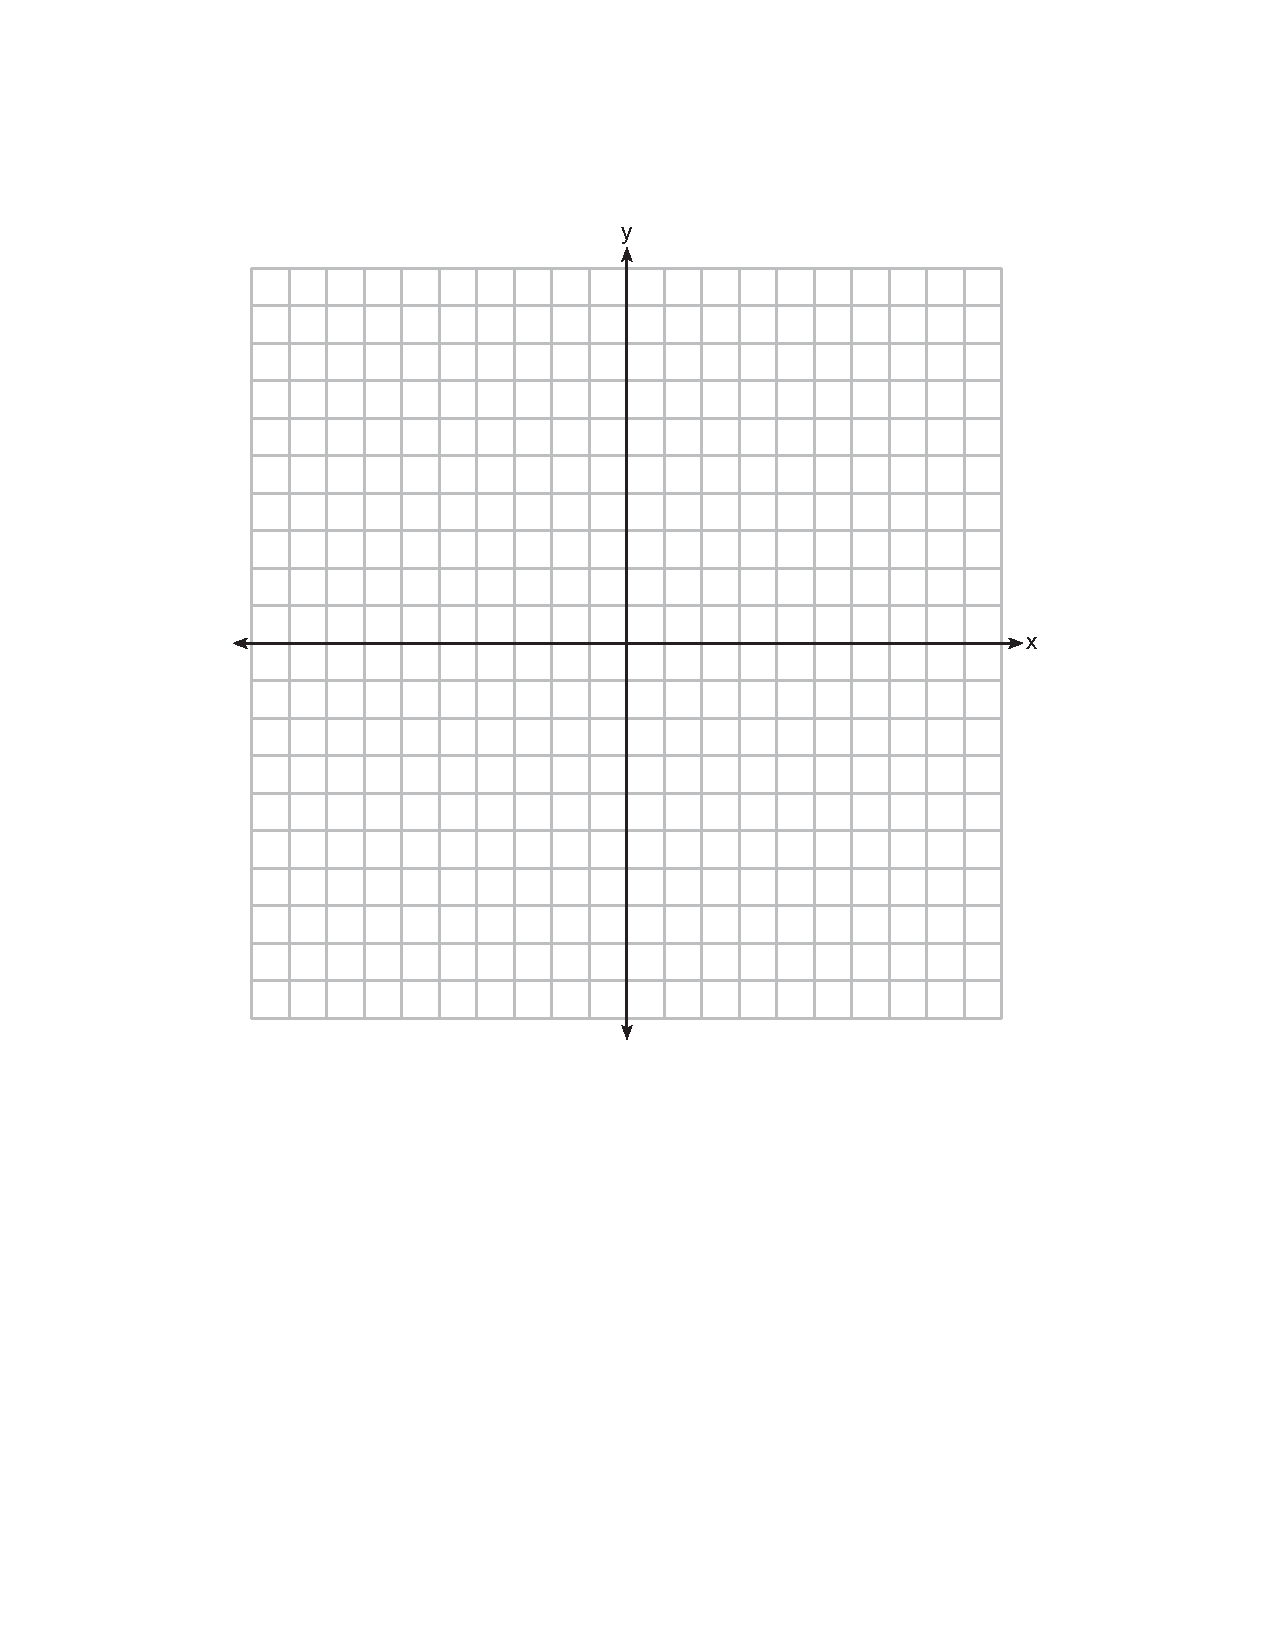
\includegraphics[width=0.75\textwidth]{regents-grid.pdf}
\end{figure}

\end{enumerate}

\end{document}
